\documentclass[b5paper,10pt,twoside]{book}
\usepackage[inner=1.5cm,outer=2cm,tmargin=1.5cm,bmargin=2cm]{geometry}

\usepackage[utf8]{inputenc}
\usepackage[spanish]{babel}
\usepackage{subfiles}
\usepackage{fancyhdr}
\usepackage[nottoc]{tocbibind}
\usepackage[square,numbers]{natbib}
\usepackage{graphicx}
\graphicspath{ {images/} }
\bibliographystyle{abbrvnat}

\pagestyle{fancy}
\fancyhf{}
\fancyhead[L]{Diario de un superviviente}

\fancyfoot[LE,RO]{\thepage}

\title{Proyecto Fin carrera}
\author{Fernando Santa Olaya Rodríguez \\
	\and 
	Rubén Toquero González}

\date{Septiembre, 2015}

\begin{document}
	\maketitle
	
	\chapter*{Agradecimientos}
	\textit{A pepito porque lo quiero con locura blabla bla} Queda formatearlo a la derecha y  formatear bien los títulos
	

	\chapter*{Resumen}
	 	El presente proyecto implementa una aplicación móvil como micro asistente virtual a personas que padezcan la lacra moderna del cáncer y una aplicación en servidor con la que se comunica la app y recopila estadísticas de actividades y estados de animo de los usuarios para su posibles estudios relacionados con la enfermedad. Ademas provee de una plataforma con la que se puede interactuar fácilmente con los usuarios de la misma por un operador de la misma. 
	 	
	\begin{figure}[h]
		\centering
		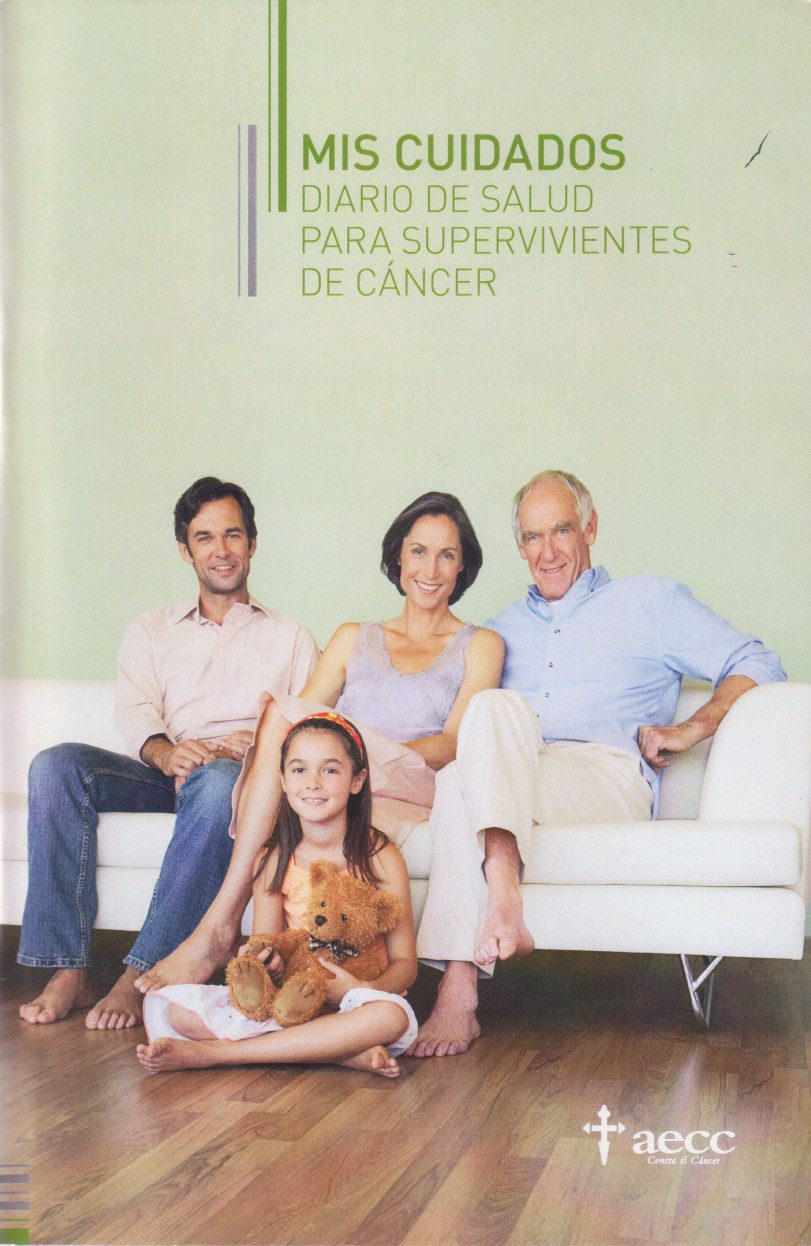
\includegraphics[width=0.25\textwidth]{fotointro}
		\caption{Portada del folleto.}
		\label{fig:mesh1}
	\end{figure}
	 
	\chapter*{Abstract}
	 	This project implents an mobile app wich is an micro virtual assitant for those people who are suffering the modern doom of cancer and on the other hand a server aplication which comunicates with the app on order to acquire data for statistic uses of the data involved with this illnes.\cite{SHAREESP}
	
	\tableofcontents
	
	\listoffigures
	
	\listoftables
	
	\chapter{INTRODUCCIÓN}
	
	\subfile{./1-Introduccion/introduccion}
	
	\chapter{Visión general del Proyecto}

	\subfile{./2-Vision/vision}
	
	\chapter{Análisis y Metodología}
	
	\subfile{./3-Analisis/analisis}
	
	\chapter{Planificación}
	
	\subfile{./4-Planificacion/planificacion}
	
	\chapter{Diseño}
	
	\subfile{./5-Diseno/diseno}
	
	\chapter{Pruebas}
	
	\subfile{./6-Pruebas/pruebas}
	
	\chapter{Conclusiones y trabajo futuro}
	
	\subfile{./7-Conclusiones/conclusiones}
	
		
	\bibliography{bibliography}

\end{document} 